\documentclass[11pt,a4paper]{article}

\usepackage{graphicx, latexsym}
\usepackage{setspace} 
\usepackage[natbibapa]{apacite}
\usepackage{amssymb, amsmath, amsthm}
\usepackage{caption, subcaption}
\usepackage{footnote}
\usepackage{authblk}
\usepackage{wrapfig,lipsum,booktabs}
\usepackage{epstopdf}
\usepackage[margin=0.98in]{geometry}
\usepackage{tikz}
\usepackage{listings}
\usepackage{pdflscape}
\usepackage{blkarray}
\usetikzlibrary{decorations.pathreplacing}
\usetikzlibrary{positioning}
\usepackage[]{hyperref}
\hypersetup{
    pdftitle={Manuscript},
    pdfauthor={Rianne Schouten},
    pdfsubject={Amputation, Imputation, Missing Data},
    pdfkeywords={Amputation, Imputation, Missing Data},
    bookmarksnumbered=true,     
    bookmarksopen=true,         
    bookmarksopenlevel=1,       
    colorlinks=true,     
    citecolor=black,    
    linkcolor=black,   
    pdfstartview=Fit,           
    pdfpagemode=UseOutlines,      
    pdfpagelayout=TwoPageRight
}

\onehalfspacing
\newcommand{\code}[1]{\texttt{#1}}

\begin{document}

\title{\LARGE\bf Generating missing values for simulation purposes:\\ A multivariate amputation procedure}

\author[1,2]{Rianne Schouten\thanks{Correspondence to: Rianne Schouten, Leuvenplein 238, 3584 LM Utrecht, the Netherlands. E-mail: r.m.schouten@uu.nl}}
\author[1]{Peter Lugtig}
\author[1]{Gerko Vink}
\affil[1]{\small University of Utrecht, Department of Methodology and Statistics, Sjoerd Groenman building, Padualaan 14, 3584 CH Utrecht, The Netherlands}
\affil[2]{\small DPA Professionals, Business Unit DPA IT, Team Data Science, Gatwickstraat 11, 1043 GL Amsterdam, The Netherlands}

\date{}
\maketitle

\begin{abstract}

Missing data form a ubiquitous problem in scientific research, especially since most statistical analyses require complete data. To evaluate the performance of methods dealing with missing data, researchers perform simulation studies. An important aspect of these studies is the generation of missing values in a simulated, complete data set: the amputation procedure. We investigated the methodological validity and statistical nature of both the current amputation practice and a newly developed and implemented multivariate amputation procedure. We studied the performance of these methods and found that the current way of practice may not be appropriate for the generation of intuitive and reliable missing data problems. That is to say, important missing data characteristics such as the missingness percentage and the impact on statistical estimates influence each other. On the other hand, we demonstrate that the multivariate amputation procedure generates reliable amputations and allows for a proper regulation of missing data problems. The procedure has additional features to generate any missing data scenario precisely as intended. Hence, the multivariate amputation procedure is an efficient method to accurately evaluate missing data methodology.

\end{abstract}

\section{Introduction}

Missing data form a ubiquitous problem in scientific research, especially since most statistical analyses require complete data. Of all possible methods for dealing with missing data (e.g. weighting procedures, likelihood based methods), multiple imputation is an appealing solution since it results in complete data sets without losing information. This is because multiple imputation replaces the missing values with estimated values based on the observed data \citep{Rubin1987, Rubin1996, Stef2012}. Because multiple imputation is now available in several statistical software packages such as SPSS, Stata, SAS and R, the application of multiple imputation has become straightforward. 

For a proper usage of methods dealing with missing data, a thorough and valid evaluation of the performance of these methods is vital. Because scientific research increasingly relies on missing data methodologies, it is important to understand under which circumstances a certain technique can and should be used. In addition, new missing data methods are continuously being developed and improved (e.g. \citealp{Vink2013}; \citealp{Fang2016}; \citealp{Kombo2016}). An accurate evaluation procedure is essential to know whether such a methodology functions properly. In this paper, we will focus on the process of generating missing values; a key procedure in the evaluation of the performance of missing data techniques. 

In general, a missing data methodology is evaluated by means of simulations. Such simulation studies generally have four steps: 

\begin{enumerate} 
\item A multivariate, complete data set is simulated and considered the population of interest. 
\item This data set is then made incomplete. 
\item The incomplete data are estimated by means of the missing data method. 
\item Statistical inferences are obtained for the original, complete data set and after dealing with the missing values. A comparison of these inferences gives an indication of the performance of the missing data method. 
\end{enumerate}

\noindent A key part in the evaluation of a missing data methodology is step 2; the generation of missing values. We refer to the process where missingness is induced in complete data as \textit{amputation}. 

In current simulation studies, missing values are generated one variable at a time. With this univariate amputation approach, it can be difficult to appropriately control the characteristics of a missing data problem. For instance, \citet[][p. 11]{Seaman2012} intended to generate missing values for 70\% of the cases, but as a result of their approach 77\% of the cases were made incomplete. Another issue, that we will return to, is that the missing data structures do not reflect what was intended by the researcher. As a result, missing data methods may be evaluated under the wrong conditions and invalid conclusions about their inferential performance may be drawn. 

A valid amputation procedure is critical for the evaluation of missing data methods as it defines the missing data problem. Hence, we will put the methodological validity and the statistical nature of the current amputation practice under close investigation. Further, we will outline an alternative approach for generating any kind of missingness in any data set. Because our amputation procedure generates missing values in a multivariate way, issues with unreliable and inconsistent missing data generation can be overcome. Additionally, to make the multivariate amputation procedure available to a broad audience, we implemented the methodology as the function \code{ampute} \citep{AmputeVignette} in R-package \code{mice} \citep{Stef2011}. 

In the next section, we will explore the way researchers currently generate missing values (section \ref{current}) and the reason why this approach may be inappropriate for generating reliable missing data problems \eqref{problems}. We will then explain the methodology of the multivariate amputation procedure \eqref{method} and detail our argument that the multivariate amputation method overcomes the problems with the current practice \eqref{solution}. Furthermore, we will demonstrate the performance of \code{ampute} with simulation research (section \ref{evaluation}) and make its improvement on the current practice evident (section \ref{compare}). We will conclude and discuss additional applications of \code{ampute} in section \ref{conclusion}. 

\section{Univariate amputation}

\subsection{\normalsize Univariate amputation}\label{current}

In current evaluations of missing data methodologies, every researcher has to develop an ad-hoc approach to generating missing values. Most of these amputation methods are designed for a particular data set. For instance, \citet[][p. 4]{Sullivan2016} simulated data ``from the model $Y_i = 0.30T_i + \beta_2X_i + e_i$, with $X$ and $e \sim N(0, 1)$'' while others use real data such as ``the complete SHS data set [with variables] age, gender, history of diabetes, CVD status, and three serial measures of Scr [i.e. serum creatinine]'' \citep[][p. 3]{Shara2015}. Because the variables of these data sets have a specific covariance structure and tailor-made amputation approaches are used, the missing data situations these researchers study are unique.

All ad-hoc amputation techniques have in common that missing values are generated in a univariate way. Univariate amputation means that missingness is generated one variable at a time. For example, \citet{Sullivan2016} generated missing values in variable $Y$. For \citet[][p. 3]{Shara2015}, ``the outcome variable of interest was CVD'' and variable Scr was the incomplete variable. 
In almost all real datasets, missingness is present for multiple variables. When such a situation needs to be mimicked in a simulation study, researchers repeatedly use a univariate amputation procedure for every variable that needs missing values. Missing values are generated first in $Y_1$, second in $Y_2$, and so on. In other words, the missingness on one variable is generated separately and independently from the missingness on any other variable. An example is the simulation study of \citet[][p. 3]{Kontopantelis2017} who describe that ``In the MAR setting, the probability to be missing for each of X, Y or Y' was independently set to be conditional on the exposure E with OR = 5.'' Other examples of studies where this procedure is followed are \citet{Abrahantes2011}, \citet{Kalaycioglu2016}, \citet{Pastor2003}. From here on, we will continue to refer to this class of approaches as \textit{stepwise univariate amputation}.

\subsection{\normalsize Problems with stepwise univariate amputation}\label{problems}

Probabilities to be missing on one or multiple variables can be independent, be related to eachother, or depend on values of covariates, or the variables themselved. The situation where the missingness does nto depend on any other variable in the datsset is referred to Missing Completely At Random \citep[i.e. MCAR,][]{Rubin1976}. Alternatively, the probability of being missing in a certain variable, say $Y_1$, can be based on the values of another variable, say $X_1$. This situation is called Missing At Random \citep[i.e. MAR,][]{Rubin1976}. \citet[][pp. 63, 64]{Stef2012} advised to relate the missingness on variable $Y_1$ to the values of $X_1$ by means of a continuous probability function, such as a logistic distribution function. However, in practice it is common to use the $X_1$ values to divide the participants into groups. Then, a specific probability value is specified for each of these groups (e.g. \citealp{Kontopantelis2017}; \citealp{Allison2000}; \citealp{Yuan2012}). A third type of missing data problem is created when the missingness in a variable is based on the variable values themselves. In that situation, the probability of a case being missing in variable $Y_1$ depends on its value on $Y_1$. We call this a Missing Not At Random mechanism \citep[i.e. MNAR,][pp. 31, 32]{Rubin1987, Stef2012}. In practice, researchers aim at generating at least one of the three missingness mechanisms to evaluate missing data methodology.

Problems with stepwise univariate amputation appear especially - but not only - when multiple variables are amputed. The stepwise univariate amputation method is problematic for a proper regulation of the characteristics of missing data problems. For instance, consider a simple characteristic of any missing data problem: the percentage of cases with missing values. When a researcher generates 50\% MCAR missing values in variable $Y_1$, each case has a probability of 0.5 of being missing in $Y_1$. When the same procedure is followed for a second variable, say $Y_2$, the probability that a case has missing values on both $Y_1$ and $Y_2$ is $0.5 \cdot 0.5 = 0.25$. Hence, to reach a certain overlapping missingness percentage, a different individual probability has to be used. Fortunately, with MCAR missingness it is quite straightforward to estimate that probability (see Appendix A.1).

\begin{figure}[t!]
\centering
\includegraphics[width=0.8\textwidth]{types_shifted.pdf}
\caption{\small Standard ($b = 0$) and shifted ($b = 0.922$) right-tailed logistic distribution functions}
\label{types_shifted}
\end{figure}

With MAR missingness, on the other hand, it is challenging to determine how the probabilities should be adapted. For example, consider a situation where we induce missingness in variables $Y_1$ and $Y_2$ and base our amputations on the values of a normally distributed variable $X_1$. When we use the standard right-tailed logistic distribution function of Figure \ref{types_shifted}, we will induce 50\% missingness in variable $Y_1$ and 50\% in variable $Y_2$. However, the joint missingnes percentage (i.e. the percentage of cases with missing values on both $Y_1$ and $Y_2$) will become 29\% instead of the intuitive 25\% (Appendix A.2). To obtain the desired missingness percentage, we can move the logistic distribution function horizontally. For instance, the right-tailed distribution function can be shifted with 0.922 (Figure \ref{types_shifted}) which will result in 50\% joint missingness (Appendix A.2). Unfortunately, this calculation requires extensive mathematical knowledge and becomes even more complicated when missingness is created in three or more variables. 

Moreover, any shift of the logistic distribution function also influences other parameters of the missing data problem, such as the impact of the missing values on the statistical outcome. Since the logistic distribution function has an asymptote at $y = 1$, a certain part of the distribution of $Y$ will almost definitely be amputed. With the right-tailed distribution function, cases with extreme $X_1$ values will have $P(\text{missing}) = 0.99$. Depending on the correlation between $X_1$ and $Y_1$, this means that high $Y_1$ values will almost certainly be made missing. When the logistic distribution function is shifted, not only will more values be amputed, but the largest part of these missings will occur in the right tail of the distribution of $Y_1$. This causes the observed distribution of $Y_1$ to become more skewed than initially intended. 

When researchers are not aware of the consequences of using a stepwise univariate amputation procedure, simulation results may not be interpreted in the right context. For instance, when missingness is created in a data set with low correlations, intended MAR missingness patterns may more reflect a MCAR mechanism \citep{Vink2016}. In such situations, the performance of the missing data method may be evaluated as sufficient when in fact the evaluation procedure - and not the missing data method - leads to the finding. The opposite could be true as well, when a researcher shifts the right-tailed logistic distribution function to the left to obtain a certain multivariate missingness percentage, but is not aware that this shift increases the severity of the MAR mechanism. Hence, the missing data method may be falsely categorized as underperforming.

\section{Multivariate amputation}

\subsection{\normalsize Multivariate amputation}\label{method}

In an ideal situation, a missing data methodology is tested with a realistic missing data problem. For the generation of multivariate missing data scenarios that mimic real-life missingness, \citet[][pp. 110 - 113]{Jaap1999} proposed an idea for a multivariate amputation that has only been briefly discussed twice \citep{Stef2006, Jaap2003}. We build upon this method and in this paper develop an amputation procedure that can generate sophisticated missing data problems. 

Figure \ref{scheme} shows a schematic overview of the resulting  multivariate amputation procedure. The procedure requires a multivariate, complete data set of $n$ participants and $m$ variables. The result of the procedure, as can be seen on the right hand side of Figure \ref{scheme}, consists of multiple subsets with either incomplete or complete data. These subsets are merged to obtain an incomplete version of the original data set. 

The amputation procedure starts with the researcher deciding what kind of missing data patterns he desires to establish. A missing data pattern is a particular combination of variables with missing values and variables remaining complete. For instance, a researcher may wish for some participants to have missing values on the first two variables, while for other participants values should be missing on variables 1 and 3. A practical example of a missing data pattern is a situation where some participants do not show up for the second round of a longitudinal study. Hence, part of the cases should have missing values on specifically the variables of the second wave. 

Based on the number of missing data patterns $k$, the complete data set is randomly divided into $k$ subsets. The size of these subsets may vary. For example, we can assign a frequency value of $\frac{2}{3}$ to a first missing data pattern and a value of $\frac{1}{3}$ to a second missing data pattern. As a result, $\frac{2}{3}$ of the cases becomes part of subset 1. 

\begin{landscape}

\thispagestyle{empty}
\begin{figure}
\hspace*{-1cm}
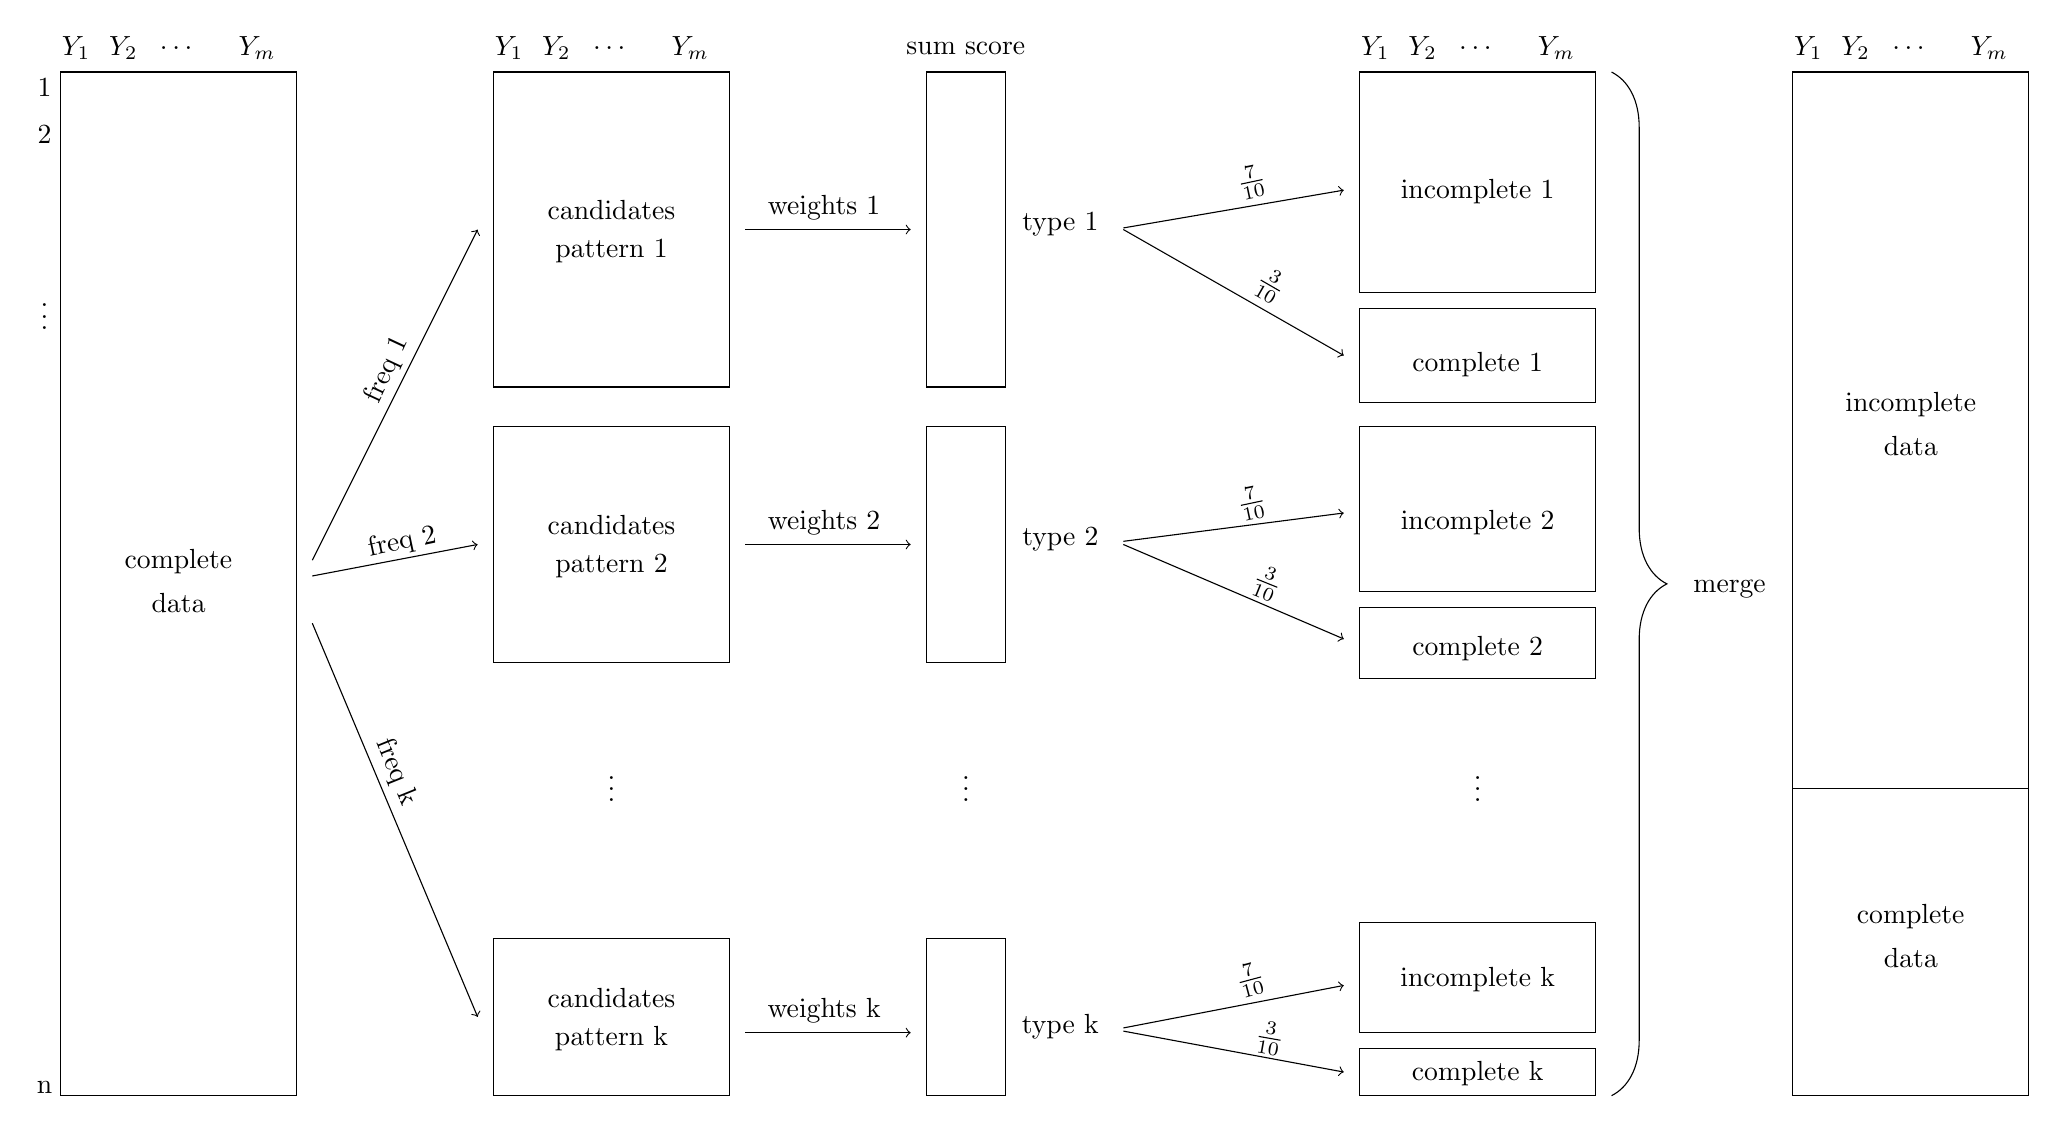
\begin{tikzpicture}

\node at (-0.2, 12.8) {1};
\node at (-0.2, 12.2) {2};
\node at (-0.2, 10) {$\vdots$};
\node at (-0.2, 0.1) {n};

\node at (0.2, 13.3) {$Y_1$};
\node at (0.8, 13.3) {$Y_2$};
\node at (1.5, 13.3) {$\dots$};
\node at (2.5, 13.3) {$Y_m$};

\draw[black] (0, 0) rectangle (3, 13);

\node [above] at (1.5, 6.5) {complete};
\node [below] at (1.5, 6.5) {data};

\draw[black] (5.5, 0) rectangle (8.5, 2);
\draw[black] (5.5, 9) rectangle (8.5, 13);
\node at (7, 4) {$\vdots$};
\draw[black] (5.5, 5.5) rectangle (8.5, 8.5);

\node [above] at (7, 11) {candidates};
\node [above] at (7, 7) {candidates};
\node [above] at (7, 1.0) {candidates};
\node [below] at (7, 11) {pattern 1};
\node [below] at (7, 7) {pattern 2};
\node [below] at (7, 1.0) {pattern k};

\node at (5.7, 13.3) {$Y_1$};
\node at (6.3, 13.3) {$Y_2$};
\node at (7, 13.3) {$\dots$};
\node at (8, 13.3) {$Y_m$};

\draw [->] (3.2, 6.8) -- (5.3, 11);
\draw [->] (3.2, 6.6) -- (5.3, 7);
\draw [->] (3.2, 6.0) -- (5.3, 1);

\node [above, rotate=65] at (4.4, 9.1) {freq 1};
\node [above, rotate=12] at (4.4, 6.75) {freq 2};
\node [above, rotate=-68] at (4.0, 4) {freq k};

\draw[black] (11, 0) rectangle (12, 2);
\draw[black] (11, 9) rectangle (12, 13);
\node at (11.5, 4) {$\vdots$};
\draw[black] (11, 5.5) rectangle (12, 8.5);

\node at (11.5, 13.3) {sum score};

\draw [->] (8.7, 11) -- (10.8, 11);
\draw [->] (8.7, 7.0) -- (10.8, 7.0);
\draw [->] (8.7, 0.8) -- (10.8, 0.8);

\node [above] at (9.7, 11) {weights 1};
\node [above] at (9.7, 7) {weights 2};
\node [above] at (9.7, 0.8) {weights k};

\draw[black] (16.5, 0) rectangle (19.5, 0.6);
\draw[black] (16.5, 0.8) rectangle (19.5, 2.2);
\draw[black] (16.5, 8.8) rectangle (19.5, 10);
\draw[black] (16.5, 10.2) rectangle (19.5, 13);
\node at (18, 4) {$\vdots$};
\draw[black] (16.5, 5.3) rectangle (19.5, 6.2);
\draw[black] (16.5, 6.4) rectangle (19.5, 8.5);

\node [above] at (18, 11.2) {incomplete 1};
\node [above] at (18, 9) {complete 1};
\node [above] at (18, 7) {incomplete 2};
\node [above] at (18, 5.4) {complete 2};
\node [above] at (18, 1.2) {incomplete k};
\node [above] at (18, 0) {complete k};

\node at (16.7, 13.3) {$Y_1$};
\node at (17.3, 13.3) {$Y_2$};
\node at (18, 13.3) {$\dots$};
\node at (19, 13.3) {$Y_m$};

\node[above] at (12.7, 10.8) {type 1};
\node[above] at (12.7, 6.8) {type 2};
\node[above] at (12.7, 0.6) {type k};

\node [above, rotate=12] at (15.2, 11.28) {$\frac{7}{10}$};
\node [above, rotate=12] at (15.2, 7.2) {$\frac{7}{10}$};
\node [above, rotate=15] at (15.2, 1.15) {$\frac{7}{10}$};
\node [above, rotate=-30] at (15.2, 10) {$\frac{3}{10}$};
\node [above, rotate=-22] at (15.2, 6.2) {$\frac{3}{10}$};
\node [above, rotate=-10] at (15.3, 0.4) {$\frac{3}{10}$};

\draw [->] (13.5, 11.02) -- (16.3, 11.5);
\draw [->] (13.5, 11.00) -- (16.3, 9.4);
\draw [->] (13.5, 7.04) -- (16.3, 7.4);
\draw [->] (13.5, 7.00) -- (16.3, 5.8);
\draw [->] (13.5, 0.86) -- (16.3, 1.4);
\draw [->] (13.5, 0.82) -- (16.3, 0.3);

\draw [decorate,decoration={brace, amplitude=20pt, mirror, raise=0pt},yshift=0pt]
(19.7,0) -- (19.7, 13); 

\node [above] at (21.2, 6.2) {merge};

\draw[black] (22, 0) rectangle (25, 3.9);
\draw[black] (22, 3.9) rectangle (25, 13);
\draw[black] (22, 0) rectangle (25, 13);

\node [above] at (23.5, 8.5) {incomplete};
\node [below] at (23.5, 8.5) {data};

\node [above] at (23.5, 2) {complete};
\node [below] at (23.5, 2) {data};

\node at (22.2, 13.3) {$Y_1$};
\node at (22.8, 13.3) {$Y_2$};
\node at (23.5, 13.3) {$\dots$};
\node at (24.5, 13.3) {$Y_m$};

\end{tikzpicture}
\caption{Schematic overview of the multivariate amputation procedure}
\label{scheme}
\end{figure}
\end{landscape}

\begin{figure}[t!]
\centering
\includegraphics[width=0.8\textwidth]{types.pdf}
\caption{\small Four variants of the logistic distribution function \citep[based on][p. 64]{Stef2012}}
\label{types}
\end{figure}

\noindent These participants are then called \textit{candidates} for missing data pattern 1. Since all cases are allocated to a subset and every case is candidate for one pattern only, the sum of the frequency values should be 1. Note that at this stage it is not yet decided whether the participants will receive missing values; they are merely \textit{candidates} for one of the $k$ missing data patterns.  

Before we explain how to calculate a so-called weighted sum score for each candidate, it is important to know that the weighted sum scores are used to determine whether a data cell becomes missing or not: based on his weighted sum score, each candidate receives a probability of being missing for a given variable. For the allocation of these probabilities, we apply one of four possible logistic distribution functions on the weighted sum scores (Figure \ref{types}). It is possible to choose a different logistic distribution function for every missing data pattern. For instance, if a right-tailed (RIGHT) type of missingness is used, candidates with high weighted sum scores will receive a high probability of being missing. With a left-tailed (LEFT), centered (MID) or both-tailed (TAIL) missingness type, higher probability values are given to the candidates with low, average or extreme weighted sum scores respectively. Since the weighted sum scores determine the  missingness probabilities, the calculation of weighted sum scores is an important part of the amputation procedure. 

Weighted sum scores are calculated as the outcome of a linear regression equation where the coefficients are determined by the researcher. The weighted sum score of case $i$ is calculated as follows:
\begin{equation*}
wss_i = w_1 \cdot y_{1i} + w_2 \cdot y_{2i} + ... + w_m \cdot y_{mi},
\end{equation*}

\noindent where $\{y_{1i}, y_{2i}, ..., y_{mi}\}$ is the set of variable values of case $i$ and $\{w_1, w_2, ..., w_m\}$ are the corresponding pre-specified weights. One weight per variable governs the impact of that variable on the formation of the sum score. Variables with higher weights will have a larger influence on the size of the weighted sum score than variables with lower weights. For instance, if variables $Y_1$ and $Y_2$ have weight values of 4 and 2 respectively, the importance of $Y_1$is twice as large as that of $Y_2$. The sign of the weight values influences whether a weighted sum score increases or decreases. A positive weight will increase the weighted sum score while a negative weight will have a decreasing effect. Furthermore, the weight values can value by missing data pattern. For example, variable $Y_1$ can have a weight value of 4 in the first pattern, but a weight value of -2 in the second pattern. 

An important feature of the multivariate amputation procedure lies in the possibility to choose a weight value of zero. A zero weight indicates that the values of that variable play no role in the calculation of the weighted sum scores. Consequently, the generation of MCAR missingness can be seen as the situation where all weight values are zero. Since the probability of being missing with MAR missingness by definition depends on the values of observed variables, we can generate MAR missingness by assigning weights of zero to all variables that will be amputed. In contrast, if we choose to give a non-zero weight to one or more of the variables that will be amputed, the generated missingness mechanism becomes MNAR. In the last step of the multivariate amputation procedure, the assigned probabilities are used to generate missing values. Because we use a probabilistic model, some cases will remain complete, while other will receive missing values (Figure \ref{scheme}).

\subsection{\normalsize Benefits of multivariate amputation}\label{solution}

With the multivariate amputation approach, we have a procedure to accurately mimic realistic missingness problems. It is straightforward to define various missing data patterns, the relative occurrence of these patterns (by defining the size of the subsets) and to manipulate the total missingness percentage for different variables. By offering the possibility to specify weight values, the multivariate amputation procedure also enables the fine-tuning of missing data mechanisms. 

With the availability of R-function \code{ampute}, we deliver a means to overcome potential problems that may occur with the current way of practice. \code{ampute}'s default settings will generate 50\% MAR-RIGHT missingness. Further, all aspects of the multivariate amputation methodology as discussed above can be regulated for different types of data (categorical data will be made numeric). Moreover, a smart use of the weight matrix enables the generation of both MAR and MNAR mechanisms within the same data set. These and other features of \code{ampute} ensure the generation of complex - but realistic - missing data problems. For a detailed explanation about \code{ampute}'s arguments, we refer to \citet{AmputeVignette}.

The next two sections will answer two research questions. First, we will evaluate the performance of \code{ampute}. By means of a simulation study, we will study whether \code{ampute} generates legitimate missingness mechanisms. Next, section \ref{compare} will compare the performance of stepwise univariate amputation and multivariate amputation. 

\section{Evaluation of \code{ampute}}\label{evaluation}

\subsection{Simulation conditions}

We perform a model-based simulation by repeatedly drawing $N = 1,000$ cases from a multivariate normal distribution with \code{mvrnorm} in the package \code{MASS} \citep{MASS} in \code{R} \citep{R}. We use mean structure

\begin{equation*}
\mu = 
\begin{blockarray}{cc}
\begin{block}{c(c)}
Y_1&5\\
Y_2&5\\
X_1&10\\
\end{block}
\end{blockarray}\hspace{1mm},
\end{equation*} 

\noindent and covariance structure  

\begin{equation*}
\Sigma = 
\begin{blockarray}{ccccc}
& Y_1 & Y_2 & X_1\\
\begin{block}{c(cccc)}
Y_1 & 1 & \rho & \rho \\
Y_2 & \rho & 1 & \rho \\
X_1 & \rho & \rho & 1 \\
\end{block}
\end{blockarray}\hspace{1mm}. 
\end{equation*}

\noindent We vary the correlation $\rho \in \{0.1, 0.2, \dots, 0.9\}$. The number of Monte Carlo simulations is 1,000.

We will examine the five different missing data scenarios from Table \ref{cond1}. For each scenario, we will generate joint missingness in variables $Y_1$ and $Y_2$ for 20\% of the cases. Note that this means that there are no cases with missing values on either $Y_1$ or $Y_2$. Rather, a case is complete or has missing values on the two $Y$ variables together. We leave $X_1$ an observed covariate (Table \ref{cond1}). 

We categorize the five missing data scenarios as a MCAR, MAR, weak MAR, MNAR and weak MNAR kind of missingness. With MCAR missingness, the probability of being missing is 0.2 for each case. For the MAR and MNAR scenarios, the probabilities of being missing are based on the values of $X_1$ and $Y_1$ respectively, indicated by $1$ in weights column in Table \ref{cond1}. In case of weak MAR missingness, one part of the cases will be MCAR while the other part is based on the values of $X_1$. For the weak MNAR simulation condition, the weighted sum scores are determined by variables $Y_1$ and $X_1$ with ratio 1:5. For all scenarios, we generate right-tailed (RIGHT) missingness as displayed in Figure \ref{types}. 

\begin{table}[b!]
\centering
\captionsetup{justification=justified,singlelinecheck=false,width = 0.50\textwidth}
\caption{\normalsize{Five simulation conditions for the evaluation of \code{ampute}}}
  \label{cond1}
\begin{tabular}{rrrrrrrrr}
  \hline
&& \multicolumn{3}{c}{pattern} && \multicolumn{3}{c}{weights} \\
\cline{3-5} \cline{7-9}
condition & & $Y_1$ & $Y_2$ & $X_1$ & & $Y_1$ & $Y_2$ & $X_1$ \\
\hline 
mcar & & 0 & 0 & 1 && 0 & 0 & 0 \\ [0.2cm]
mar & & 0 & 0 & 1 && 0 & 0 & 1 \\ [0.2cm]
weak mar & & 0 & 0 & 1 && 0 & 0 & 0 \\ 
 & & 0 & 0 & 1 && 0 & 0 & 1 \\[0.2 cm]
mnar & & 0 & 0 & 1 && 1 & 0 & 0 \\ [0.2cm]
weak mnar & & 0 & 0 & 1 && 1 & 0 & 5\\
   \hline
   \end{tabular}
   \vspace{2mm}
   \captionsetup{justification=justified,singlelinecheck=false,width = 0.50\textwidth}
\caption*{\footnotesize{\textit{Note.} The pattern column displays whether variables are amputed ($0$) or remain complete ($1$). The weights column displays whether the variables influence the amputations.}}
\end{table}

For reasons of brevity, we focus our evaluation on the mean value of $Y_1$ ($\mathbb{E}_{Y_1}$). We calculate $\mathbb{E}_{Y_1}$ for every incomplete data set with complete case analysis (CCA) and after multiple imputation (MI) with predictive mean matching as the imputation technique (PMM; \code{mice.impute.pmm}). This last step, of imputing the variables again, is crucial to see whether exisiting missing data methodologies can recover the missing data we generate.
For every replication, we generate $m = 5$ multiply imputed data sets and combine the $m$ completed data means into a single inference following Rubin's rules \citep[][pp. 76, 77]{Rubin1987}.

We study the coverage rate of the 95\% confidence intervals for the mean (i.e. in how many of the 1,000 replications does the 95\% confidence interval of $\mathbb{E}_{Y_1}$ contain the true population value of $\mathbb{E}_{Y_1} = 5$), the average width of that confidence interval and the average bias with respect to the true population value of $\mathbb{E}_{Y_1} = 5$. 

\subsection{\normalsize Hypotheses}\label{hypotheses}

When MCAR missingness is generated, the observed distribution of $Y_1$ will be thinned. Consequently, CCA will yield unbiased estimates and the coverage rates will be around 0.95. When the MAR and MNAR mechanisms are generated as intended, CCA estimates will be negatively biased and the coverage rates will be under 0.95. Because we induced right-tailed missingness, the right side of the distribution of $Y_1$ will be amputed. As a result, the observed distribution of $Y_1$ becomes skewed which leads to a negative bias in the CCA estimates of $\mathbb{E}_{Y_1}$. The same holds for the weak MAR and weak MNAR simulation conditions. 

Because we know that MI yields valid inference when the observed data contains the information about the missing part, we expect that after imputation, estimates of $\mathbb{E}_{Y_1}$ are unbiased and efficient for the MCAR, MAR and weak MAR simulation conditions. In case of MNAR missingness, the information about the true data model is not available from the observed data. Thus, a MNAR missingness mechanism will still give biased estimates and coverage rates will be under 0.95. For the same reason, weak MNAR missingness will yield invalid statistical inferences, but because the observed information of the weak MAR condition partly contains the information about the missing values, the deviation from the true population value may be smaller than with MNAR missingness. 

\subsection{Results}

\begin{figure}[t!]
\begin{subfigure}{.51\textwidth}
\includegraphics[width = 1.0\linewidth]{Figure1a.pdf}
\vspace{-2.2\baselineskip}
\subcaption{}
\label{01a}
\end{subfigure}
\vspace{-1.1\baselineskip}
\begin{subfigure}{.51\textwidth}
\includegraphics[width=1.0\linewidth]{Figure1b.pdf}
\vspace{-2.2\baselineskip}
\subcaption{}
\label{01b}
\end{subfigure}
\vspace{-1.1\baselineskip}
\begin{subfigure}{.51\textwidth}
\includegraphics[width = 1.0\linewidth]{Figure1c.pdf}
\vspace{-2.2\baselineskip}
\subcaption{}
\label{01c}
\end{subfigure}
\begin{subfigure}{.51\textwidth}
\includegraphics[width=1.0\linewidth]{Figure1d.pdf}
\vspace{-2.2\baselineskip}
\subcaption{}
\label{01d}
\end{subfigure}
\begin{subfigure}{.51\textwidth}
\includegraphics[width = 1.0\linewidth]{Figure1e.pdf}
\vspace{-2.2\baselineskip}
\subcaption{}
\label{01e}
\end{subfigure}
\begin{subfigure}{.51\textwidth}
\includegraphics[width=1.0\linewidth]{Figure1f.pdf}
\vspace{-2.2\baselineskip}
\subcaption{}
\label{01f}
\end{subfigure}
{\caption{\normalsize Evaluation of R-function \code{ampute}. Coverage rate, bias and confidence interval width of $\mathbb{E}_{Y_1}$ estimates are shown for complete case analysis (a, c, e) and multiple imputation by predictive mean matching (b, d, f). The x-axis shows the data correlation $\rho \in \{0.1, 0.2, \dots, 0.9\}$.}
\label{sim1}}
\end{figure}

Figure \ref{sim1} shows the coverage rate, average bias and average confidence interval width of the estimates of $\mathbb{E}_{Y_1}$ for CCA and MI. We will discuss the results by examining Figures \ref{01a}/c, \ref{01b}/d and \ref{01e}/f respectively. Note that a numerical representation of this information is available from Table A in the Appendix B. 

As expected, MCAR missingness results in unbiased estimates (Figure \ref{01a}) and coverage rates around 0.95 (Figure \ref{01c}). In line with our hypotheses, all MAR and MNAR missingness mechanisms produce negatively biased estimates (Figure \ref{01a}) and cause a drop in the coverage rates (Figure \ref{01c}). It is interesting to see that for missing data scenarios where $X_1$ governs the amputation procedure (i.e. with MAR, weak MAR and weak MNAR missingness), the size of the bias has a linear relation with data correlation $\rho$. This is not the case for MCAR and MNAR missingness, as these mechanisms do not depend on the values of $X_1$. 

Figures \ref{01b} and \ref{01d} show that when the observed data holds the information about the missingness (i.e. with MCAR, weak MAR and MAR missingness), MI results in unbiased estimates and coverage rates around 0.95. In contrast, when the missingness is based on the missing values themselves (i.e. with weak MNAR and MNAR missingness), the estimates of $\mathbb{E}_{Y_1}$ are biased and coverage rates are under 0.95. These results are in line with what we know from theory. Furthermore, Figure \ref{01d} shows that when the correlations between $X_1$, $Y_1$ and $Y_2$ are high, the coverage rates of these mechanisms increase towards 0.95. It is promising to see that MI can utilize the observed information to solve (part of) the missing data problem. 

Because the percentage of cases with missing values is similar in all simulation conditions (20\%), the width of the 95\% confidence interval should be seen as a measure of the variance of the observed distribution of $Y_1$. For MCAR missingness, this variance is larger than for MNAR missingness (see Figure \ref{01e}). Besides, we see that compared with CCA, the confidence interval widths after MI start with a higher value. This effect is expected because MI produces between imputation variance on top of the data variance \citep{Rubin1987}. Nonetheless, when data correlation $\rho$ increases, MI decreases the confidence interval widths (Figure \ref{01f}). In fact, the competence of MI to simultaneously reduce the bias and the variance of statistical estimates makes this missing data method the fantastic method we know it is. 

In sum, we find that \code{ampute} produces the five evaluated missing data scenarios exactly according our hypotheses. Without any doubt we can conclude that \code{ampute} produces legitimate MCAR, MAR and  MNAR missingness and any desired variation thereof. 

\section{Comparison of amputation procedures}\label{compare}

\subsection{\normalsize Simulation conditions}

To compare the performance of stepwise univariate amputation (SUA) and multivariate amputation (MA), we perform a model-based simulation study. Similar to section \ref{evaluation}, we repeatedly draw $N = 1,000$ cases from a multivariate normal distribution with the same mean and covariance structures. We vary the data correlation $\rho \in \{0.2, 0.5, 0.8\}$ and again, replicate the simulations 1,000 times. 

It is our intention to generate missing values for 50\% of the cases. The incomplete cases will have missing values on both variables $Y_1$ and $Y_2$. Note that we will not permit cases to have missing values on either $Y_1$ or $Y_2$. Rather, 50\% of the cases has joint missingness on variables $Y_1$ and $Y_2$ while the other 50\% remains complete. Besides, we leave $X_1$ to be an always observed covariate.

We compare three simulation conditions: two SUA approaches and MA. For the first SUA approach, we repeat the \textit{standard} right-tailed (RIGHT) type of logistic distribution function for variables $Y_1$ and $Y_2$ (cf. Figure \ref{types_shifted}). For the second simulation condition, we take the same approach but with a \textit{shifted} probability distribution (cf. Figure \ref{types_shifted}). We determined $b$ to be $0.922$. This can be calculated with Equation \eqref{twovariables} in Appendix A.2. Third, we jointly generate missing values for variables $Y_1$ and $Y_2$ with the implementation of MA in R-function \code{ampute}. The specifications of the arguments of the function are attached in Appendix C.

We perform simulations for both MAR and MNAR missingness. For the two SUA conditions, we distinguish between MAR and MNAR missingness by choosing either $X_1$ (MAR) or $Y_1$ (MNAR) as the x-axis variable in Figure \ref{types_shifted}. With \code{ampute}, we made the according specifications for the weight values (see Appendix C). In addition, we repeat the process for a data set with four variables ($Y_1$, $Y_2$, $Y_3$ and $X_1$) where we intent to generate 50\% joint missingness on variables $Y_1$, $Y_2$ and $Y_3$. 

Equivalent to the simulation study of section \ref{evaluation}, we evaluate the mean value of $Y_1$ ($\mathbb{E}_{Y_1}$) with complete case analysis (CCA) and after multiple imputation (MI) with predictive mean matching as the imputation technique (PMM; \code{mice.impute.pmm}). We choose for PMM because this imputation technique samples from the observed data and thus, may be more sensitive to amputing part of the true data distribution than other imputation methods \citep{Vink2014}. By comparing the actual obtained missingness percentage, the average bias, the average width of the 95\% confidence interval and the coverage rate of these intervals, we can evaluate and compare the performance of the three amputation approaches. 

\subsection{\normalsize Hypotheses}

Although we intent to generate missing values for 50\% of the cases, we expect to see that standard SUA gives a missingness percentage smaller than 50. By definition, SUA generates the missing values in $Y_1$ separately from the missingness in $Y_2$. Therefore, it is difficult to regulate the percentage of joint missingness. In contrast, as we manually shifted the distribution function for the second simulation condition, we anticipate a joint missingness percentage of 50 for this simulation condition. With MA, regulation of the missingness percentage is no issue and we expect to see a neat 50\% there as well. 

When it is the intention to generate 50\% right-tailed missingness in a normally distributed variable, the observed distribution of this variable is supposed to get a steady, fixed degree of skewness. With CCA, we can observe this level of skewness by evaluating the bias in the estimates of $\mathbb{E}_{Y_1}$. Because it is logical that the actual obtained missingness proportion is of influence on the size of this bias as well, we expect that the estimates of standard SUA will have smaller bias values than the other two simulation conditions. These small biases induce the generated missing data problem to be less severe. Furthermore, as shifting the distribution function will engender a ceiling effect (see section \ref{problems}), we expect that shifted SUA will generate too much bias in the estimates of $\mathbb{E}_{Y_1}$. Hence, shifted SUA will generate a too severe missing data problem. In contrast, MA works such that not only the intended 50\% of the cases will be made incomplete but the procedure will also produce the legitimate degree of skewness.

We examine the consequences of the three amputation approaches for the evaluation of a missing data methodology by investigating the estimates of $\mathbb{E}_{Y_1}$ after imputation. The performance of MI depends on 1) whether the observed information contains the information about the missing part and 2) the severity of the generated missing data problem. As a result of the first, we expect that for MAR missingness MI returns unbiased and efficient estimates. With a MNAR mechanism, the information about the missingness lies outside the observed data and therefore, we expect to see biased estimates. Fortunately, MI uses the observed data to reduce the bias as much as possible. Furthermore, because standard SUA produces too small biases, shifted SUA produces too large biases and MA returns the intended biases, an evaluation of the performance of MI will be too optimal for standard SUA, too pessimistic for shifted SUA and legitimate for MA.  

\subsection{\normalsize Results}\label{results2}

\begin{table}[h!]
\begin{subtable}{1\textwidth}
\centering
\captionsetup{justification=justified,singlelinecheck=false,width = 0.93\textwidth}
\subcaption*{\normalsize Table 2: Generation of MAR missingness on 2 variables with standard and shifted stepwise univariate amputation (SUA) and multivariate amputation (MA)}
  \label{sim2a}
\begin{tabular}{rrrrrrrrrrrr}
\hline
&& \multicolumn{2}{c}{\%mis} && \multicolumn{3}{c}{cca} && \multicolumn{3}{c}{mi} \\
\cline{3-4} \cline{6-8} \cline{10-12}
cor & condition & int & obt & & bias & ciw & cov & & bias & ciw & cov \\ 
\hline
 & standard SUA & 50 & 29 &  & -0.061 & 0.147 & 0.630 &  & -0.004 & 0.166 & 0.947 \\ 
  0.2 & shifted SUA & 50 & 50 &  & -0.092 & 0.175 & 0.455 &  & 0.001 & 0.223 & 0.938 \\ 
   & MA with \code{ampute} & 50 & 50 &  & -0.081 & 0.175 & 0.552 &  & -0.001 & 0.219 & 0.936 \\ 
   \cline{2-12}
   & standard SUA & 50 & 29 &  & -0.146 & 0.144 & 0.028 &  & -0.002 & 0.156 & 0.940 \\ 
  0.5 & shifted SUA & 50 & 50 &  & -0.233 & 0.172 & 0.000 &  & -0.007 & 0.204 & 0.917 \\ 
   & MA with \code{ampute} & 50 & 50 &  & -0.207 & 0.172 & 0.002 &  & -0.005 & 0.193 & 0.936 \\ 
   \cline{2-12}
   & standard SUA & 50 & 29 &  & -0.235 & 0.139 & 0.000 &  & -0.007 & 0.137 & 0.936 \\ 
  0.8 & shifted SUA & 50 & 50 &  & -0.372 & 0.164 & 0.000 &  & -0.013 & 0.157 & 0.913 \\ 
   & MA with \code{ampute} & 50 & 50 &  & -0.331 & 0.166 & 0.000 &  & -0.010 & 0.157 & 0.912 \\ 
   \hline
\end{tabular}
\vspace{2mm}
\captionsetup{justification=justified,singlelinecheck=false,width = 0.93\textwidth}
\subcaption*{\footnotesize{\textit{Note.}  Estimates of $\mathbb{E}_{Y_1}$ are evaluated with complete case analysis (cca) and multiple imputation (mi). Comparisons are done for the intended (int) and obtained (obt) missingness percentage (\%mis), the bias, confidence interval width (ciw) and coverage rate (cov) for correlations $\rho \in \{0.2, 0.5, 0.8\}$ (cor).}}
  \end{subtable}
\bigskip
\begin{subtable}{1\textwidth}
\vspace{3mm}
\centering
\captionsetup{justification=justified,singlelinecheck=false,width = 0.93\textwidth}
\subcaption*{\normalsize Table 3: Generation of MNAR missingness on 2 variables with standard and shifted stepwise univariate amputation (SUA) and multivariate amputation (MA)}
  \label{sim2b}
\begin{tabular}{rrrrrrrrrrrr}
\hline
&& \multicolumn{2}{c}{\%mis} && \multicolumn{3}{c}{cca} && \multicolumn{3}{c}{mi} \\
\cline{3-4} \cline{6-8} \cline{10-12}
cor & condition & int & obt & & bias & ciw & cov & & bias & ciw & cov \\ 
\hline
 & standard SUA & 50 & 29 &  & -0.291 & 0.134 & 0.000 &  & -0.282 & 0.142 & 0.000 \\ 
  0.2 & shifted SUA & 50 & 50 &  & -0.465 & 0.158 & 0.000 &  & -0.451 & 0.178 & 0.000 \\ 
   & MA with \code{ampute} & 50 & 50 &  & -0.415 & 0.160 & 0.000 &  & -0.401 & 0.182 & 0.000 \\ 
   \cline{2-12}
   & standard SUA & 50 & 29 &  & -0.289 & 0.134 & 0.000 &  & -0.227 & 0.137 & 0.000 \\ 
  0.5 & shifted SUA & 50 & 50 &  & -0.465 & 0.158 & 0.000 &  & -0.369 & 0.169 & 0.000 \\ 
   & MA with \code{ampute} & 50 & 50 &  & -0.412 & 0.160 & 0.000 &  & -0.325 & 0.169 & 0.000 \\ 
   \cline{2-12}
   & standard SUA & 50 & 29 &  & -0.292 & 0.134 & 0.000 &  & -0.121 & 0.129 & 0.064 \\ 
  0.8 & shifted SUA & 50 & 50 &  & -0.466 & 0.158 & 0.000 &  & -0.199 & 0.148 & 0.000 \\ 
   & MA with \code{ampute} & 50 & 50 &  & -0.415 & 0.160 & 0.000 &  & -0.175 & 0.148 & 0.009 \\ 
   \hline
\end{tabular}
\vspace{2mm}
\captionsetup{justification=justified,singlelinecheck=false,width = 0.93\textwidth}
\subcaption*{\footnotesize{\textit{Note.}  Estimates of $\mathbb{E}_{Y_1}$ are evaluated with complete case analysis (cca) and multiple imputation (mi). Comparisons are done for the intended (int) and obtained (obt) missingness percentage (\%mis), the bias, confidence interval width (ciw) and coverage rate (cov) for correlations $\rho \in \{0.2, 0.5, 0.8\}$ (cor).}}
  \end{subtable}
\bigskip
\begin{subtable}{1\textwidth}
\centering
\captionsetup{justification=justified,singlelinecheck=false,width = 0.93\textwidth}
\subcaption*{\normalsize Table 4: Generation of MAR missingness on 3 variables with standard and shifted stepwise univariate amputation (SUA) and multivariate amputation (MA)}
  \label{sim2c}
\begin{tabular}{rrrrrrrrrrrr}
  \hline
&& \multicolumn{2}{c}{\%mis} && \multicolumn{3}{c}{cca} && \multicolumn{3}{c}{mi} \\
\cline{3-4} \cline{6-8} \cline{10-12}
cor & condition & int & act & & bias & ciw & cov & & bias & ciw & cov \\ 
\hline
 & standard SUA & 50 & 19 &  & -0.042 & 0.138 & 0.776 &  & 0.001 & 0.147 & 0.950 \\ 
  0.2 & shifted SUA & 50 & 39 &  & -0.078 & 0.158 & 0.507 &  & -0.003 & 0.195 & 0.947 \\ 
   & MA with \code{ampute} & 50 & 50 &  & -0.084 & 0.175 & 0.521 &  & -0.004 & 0.221 & 0.937 \\ 
   \cline{2-12}
   & standard SUA & 50 & 19 &  & -0.108 & 0.135 & 0.128 &  & -0.002 & 0.140 & 0.942 \\ 
  0.5 & shifted SUA & 50 & 39 &  & -0.193 & 0.154 & 0.003 &  & -0.005 & 0.173 & 0.940 \\ 
   & MA with \code{ampute} & 50 & 50 &  & -0.209 & 0.172 & 0.003 &  & -0.008 & 0.196 & 0.939 \\ 
   \cline{2-12}
   & standard SUA & 50 & 19 &  & -0.172 & 0.131 & 0.001 &  & -0.004 & 0.131 & 0.951 \\ 
  0.8 & shifted SUA & 50 & 38 &  & -0.310 & 0.148 & 0.000 &  & -0.015 & 0.145 & 0.901 \\ 
   & MA with \code{ampute} & 50 & 50 &  & -0.331 & 0.166 & 0.000 &  & -0.017 & 0.155 & 0.904 \\ 
   \hline
\end{tabular}
\vspace{2mm}
\captionsetup{justification=justified,singlelinecheck=false,width = 0.93\textwidth}
\subcaption*{\footnotesize{\textit{Note.}  Estimates of $\mathbb{E}_{Y_1}$ are evaluated with complete case analysis (cca) and multiple imputation (mi). Comparisons are done for the intended (int) and obtained (obt) missingness percentage (\%mis), the bias, confidence interval width (ciw) and coverage rate (cov) for correlations $\rho \in \{0.2, 0.5, 0.8\}$ (cor).}}
  \end{subtable}
  \vspace{-3.0\baselineskip}
  \end{table}

First of all, the obtained missingness percentages are precisely as expected. Furthermore, Table 2 shows that although the missingness percentages of shifted SUA and MA are similar, there is a difference in the generated bias. For instance, when the correlations between $X_1$, $Y_1$ and $Y_2$ are $0.2$, the average bias with shifted SUA is $-0.092$ while it is $-0.081$ with MA. These findings show that although shifting the logistic distribution function results in the desired missingness percentage, the severity of the missing data problem has changed as well. In addition, the higher the correlation in the simulated data, the more apparent this effect becomes. For instance, compare the difference between $-0.233$ and $-0.207$ for $\rho = 0.5$ with the difference between $-0.372$ and $-0.331$ for $\rho = 0.8$. All these findings are in line with our hypotheses. Furthermore, Table 2 displays a relatively small confidence interval width for standard SUA ($0.147$ for $\rho = 0.2$). The other two approaches have larger and comparable confidence interval widths because their missingness percentages are larger. However, due to their difference in bias, the coverage rates of shifted SUA and MA have become different. An example of this situation occurs for $\rho = 0.2$. There, shifted SUA results in a coverage rate of $0.455$ while it is $0.552$ for MA.

What we know from theory - MI yields valid inference for MAR missing data - can clearly be seen in Table 2. MI decreases the biases to zero. Interestingly, we notice that although the missingness proportions for shifted SUA and MA are similar, the 95\% confidence intervals do not always have an equal width. Probably, our finding that shifted SUA increases the severity of the missing data problem affects the performance of MI. Based on these results, a direct consequence for the coverage rates cannot be justified. However, we do see that it is possible that the performance of MI is different for shifted SUA than for MA. For instance, the coverage rate after MI is $0.917$ for shifted SUA and $0.936$ for MA when $\rho = 0.5$.

Table 3 displays the results for MNAR missingness. Our findings are in line with our hypotheses and comparable with the trends discussed above. Further, the results presented in Table 4 confirm our hypothesis that MA enables the generation of reliable missing data problems. That is to say, when the required adaptation of the logistic distribution function is not executed, the missingness percentages of SUA quickly drop below the intended percentage. Table 4 shows that standard SUA generates missing values for merely 19\% of the cases and the shift of $b = 0.922$ induces 39\% joint missingness. In contrast, MA exactly generates the intended 50\% missingness. Moreover, we see that with MA the average bias with CCA is similar to the bias we saw earlier. Namely, when $\rho = 0.8$, the bias is $-0.331$ in Table 2 and 4. This finding shows that MA allows for the adjustment of one feature without disturbing other missing data characteristics. In sum, MA performs the amputation procedure according the intentions.

\section{Conclusion and Discussion}\label{conclusion}

\subsection{\normalsize Conclusion}

A valid amputation procedure is essential for an accurate evaluation of the performance of missing data methodology. We showed that the approach of stepwise univariate amputation may not be appropriate for the generation of intuitive and reliable missing data problems. Namely, stepwise univariate amputation does not allow for a precise manipulation of missing data characteristics. For instance, one of the most basic features of missing data problems - the missingness percentage - requires the solving of complex integrals. These calculations can be done for situations with two or three variables, but for larger data sets a proper generation of any realistic missing data problem becomes impossible. In addition, we showed that an increase of the missing data proportion leads to an inflated observed data skewness. Hence, the evaluation of missing data methodology may happen under the wrong simulation conditions and missing data methodology can be falsely judged to under- or overperform. 

We implemented a multivariate amputation procedure into R-function \code{ampute}. We showed that \code{ampute} generates any missing data scenario precisely as desired. With multivariate amputation, missing data characteristics such as the missingness percentage and the number of incomplete variables are easy to manipulate. Furthermore, the amputations induce a missing data problem which behaves exactly as intended. In other words, when MAR missingness is intended, MAR missingness is generated. Moreover, we showed that the degree of observed data skewness is not sensitive to the number of amputed variables. This indicates that multivariate amputation allows for a separate regulation of missing data parameters. All in all, the multivariate amputation procedure is an intuitive and reliable amputation method which enables valid evaluations of missing data methodology. 

\subsection{\normalsize Discussion}

Possible applications of multivariate amputation function \code{ampute} can be found in the field of survey research. Many studies describe the use of so-called planned missing data designs (e.g. \citealp{Enders}; \citealp{Wu}; \citealp{Bunting}), which are survey designs where ``missing data are used strategically to improve the validity of data collection.'' \citep[][p. 426]{Rhemtulla2012}. For instance, in order to reduce the respondent's burden, a large questionnaire is divided into multiple parts and each participant receives one or two of these parts. Such a multi-form design is almost always based on random chance (i.e. MCAR) which may give weird combinations of questions. With \code{ampute}, it is possible to create a logical combination of variables and to investigate the most efficient way to shorten a questionnaire. 

In addition, two-method measurements designs (e.g. \citealp{Graham2006}; \citealp{Rhemtulla2012}) could benefit from the availability of \code{ampute}. With this type of planned missing data designs, all participants fill in a questionnaire but only a small part of the participants is invited for a second measurement wave. Currently, the selection of these second wave participants is based on the values of one variable. As an alternative, \code{ampute} could combine the information of multiple variables. Possibly, this could enhance the use of observed information and reduce the number of participants without a loss of statistical power. 

With the availability of a multivariate amputation procedure, systematic evaluations of the performance of missing data methods are feasible. With R-function \code{ampute}, it is easy to assess in which situations which missing data methods are preferred. Besides, any usage of \code{ampute} is not restricted to evaluations of imputation techniques. Evaluations of weighting procedures (e.g. \citealp{Boeschoten2017}) and likelihood-based methods (e.g. \citealp{Little2002}; \citealp{Molenberghs2007}) can be done as well. Besides, scientific studies that examine the combination of multiple source data (e.g. \citealp{Waal2017}), different types of measurement error (e.g. \citealp{Waal2016}) or the application of missing data methods in software tools (e.g. \citealp{Horton}) could benefit from \code{ampute}.

We focused our simulations on right-tailed MCAR, MAR and MNAR missingness. Additionally, it would be interesting to know how these and variants of these mechanisms behave in data structures other than the multivariate normal distribution. For instance, what happens with the accuracy of statistical estimates when variables have a non-linear relation? And how can \code{ampute} be used to generate a realistic multilevel missing data problem? Especially the effect of correlations on the outcome of the amputation procedure may need extra attention. Because correlations determine a large part of the effect of missing values on statistical inferences, and because correlations are important for the performance of missing data methods, it would be valuable to gain more insights into this aspect of multivariate amputation. 

Overall, we emphasize the importance of a greater understanding of the behaviour of missing data mechanisms and their impact on the validity of both the generation and the handling of missing data. After all, for an accurate evaluation strategy, an efficient and reliable amputation procedure is just the beginning. 

\bibliographystyle{apacite} 
\bibliography{References}

\normalsize \section*{Appendices}

\subsection*{Appendix A.1}

Consider two discrete random variables $Z_1$ and $Z_2$ such that $z_{1i}$ is the probability of case $i$ to be missing on variable $Y_1$ and that $z_{2i}$ is the probability of case $i$ to be missing on variable $Y_2$. We give each case the same probability $p$ and we use this probability for both variables. Hence, 

\begin{equation*}
z_{1i} = z_{2i} = p \hspace{3mm} \forall i \in \{1, 2, ..., n\}. 
\end{equation*}

\noindent To know the expected proportion of missing values in $Y_1$, we calculate the expectation of $Z_1$. By definition \citep{Freund},  

\begin{equation*}
\mathbb{E}[X] = \sum_{i = 1}^n x_i \cdot f(x),  
\end{equation*}

\noindent and therefore

\begin{align*}
\mathbb{E}[Z_1] &= \sum_{i = 1}^n p \cdot \frac{1}{n} \\
&= \frac{1}{n} \cdot \sum_{i = 1}^n p \\
&= \frac{n \cdot p}{n} = p.
\end{align*}

\noindent We desire to choose $p$ such that the total percentage of cases with missing values on both variables $Y_1$ and $Y_2$ equals a certain value $m$. In other words, we desire to let $\mathbb{E}[Z_1 \cdot Z_2] = m$. By definition, because $Z_1$ and $Z_2$ are dependent, 

\begin{equation}\label{general}
\mathbb{E}[Z_1 \cdot Z_2] = \mathbb{C}ov(Z_{1}, Z_{2}) + \mathbb{E}[Z_1] \cdot \mathbb{E}[Z_2]. 
\end{equation}

\noindent Since $\mathbb{E}[Z_1] = \mathbb{E}[Z_2]$, 

\begin{equation}\label{cov}
\mathbb{C}ov(Z_{1}, Z_{2}) = \mathbb{V}ar(Z_1) = \mathbb{E}[(Z_1 - \mathbb{E}[Z_1])^2] = \mathbb{E}[{Z_1}^2] - {(\mathbb{E}[Z_1])}^2,
\end{equation}

\noindent which gives

\begin{equation}\label{similar}
\mathbb{E}[Z_1 \cdot Z_2] = \mathbb{E}[{Z_1}^2] - {(\mathbb{E}[Z_1])}^2 + \mathbb{E}[Z_1] \cdot \mathbb{E}[Z_1] =  \mathbb{E}[{Z_1}^2]. 
\end{equation}

\noindent Furthermore, by definition \citep{Freund}, 

\begin{equation*}
\mathbb{E}[X^2] = \sum_{i = 1}^n x_i^2 \cdot f(x),  
\end{equation*}

\noindent and therefore, 

\begin{align*}
\mathbb{E}[{Z_1}^2] = m &= \sum_{i = 1}^n p^2 \cdot \frac{1}{n}\\
&= \frac{1}{n} \cdot n \cdot p^2\\
&= p^2.\\
\end{align*}

\noindent Hence,

\begin{equation}\label{solve}
p = \sqrt{m}.
\end{equation}

\noindent Equation \eqref{solve} can be used to calculate the required random fixed probability. For instance, when an overlapping missingness percentage of 50\% is desired, probability $p$ should be $\sqrt{0.5} = 0.707$. 

\noindent Note that, as a consequence, the proportion of totally complete cases equals

\begin{align*}
\mathbb{E}[(1-Z_1)^2] &= \sum_{i = 1}^n {(1-\sqrt{0.5})}^2 \cdot \frac{1}{n} \\
&= \frac{1}{n} \cdot \sum_{i = 1}^n 0.293^2 \\
&= \frac{n \cdot 0.086}{n} = 0.086.
\end{align*}

\subsection*{Appendix A.2}

Let $X$ be a continuous random variable with as its probability density function, 

\begin{equation*}
f(x) = \frac{1}{\sigma\sqrt{2\pi}}\cdot e^{-\frac{1}{2}(\frac{x - \mu}{\sigma})^2}.
\end{equation*}

\noindent Furthermore, let $Z_1$ and $Z_2$ be two continuous random variables such that $z_{1i}$ is the probability of case $i$ to be missing on a variable $Y_1$ and $z_{1i}$ is the probability of case $i$ to be missing on a variable $Y_2$. We relate the values of $Z_1$ and $Z_2$ to those of $X$ by the logistic distribution function. Hence, 

\begin{equation*}
Z_1 = Z_2 = g(X) = \frac{1}{1 + e^{-\alpha X - b}}.
\end{equation*}

\noindent By definition \citep{Freund}, the expected value of $g(X)$ is given by 

\begin{equation*}
\mathbb{E}[g(X)] = \int_{-\infty}^\infty g(x) \cdot f(x) dx
\end{equation*}

\noindent and therefore, 

\begin{equation*}
\mathbb{E}[Z_1] = \int_{-\infty}^\infty \frac{1}{1 + e^{-\alpha x - b}} \cdot \frac{1}{\sigma\sqrt{2\pi}}\cdot e^{-\frac{1}{2}(\frac{x - \mu}{\sigma})^2} dx.
\end{equation*}

\noindent When we choose $\sigma = 1$ and $\mu = 0$ such that $X$ has a standard normal distribution, and choose $\alpha = 1$ and $b = 0$ such that $g(X)$ is the standard logistic function, 

\begin{align*}
\mathbb{E}[Z_1] & = \int_{-\infty}^\infty \frac{1}{1 + e^x} \cdot \frac{1}{\sqrt{2\pi}}\cdot e^{-\frac{1}{2}x^2} dx \nonumber \\
& = 0.5.
\end{align*}

\noindent In other words, the expected percentage of cases with a missing value on $Y_1$ is 50\%. The same holds for variable $Y_2$. However, the percentage of cases with missing values on both $Y_1$ and $Y_2$ will be different. Namely, in accordance with Equations \eqref{general}, \eqref{cov} and \eqref{similar}, and since 

\begin{equation*}
\mathbb{E}[{g(X)}^2] = \int_{-\infty}^\infty {g(x)}^2 \cdot f(x) dx, 
\end{equation*}

\noindent the proportion of cases with missing values on both $Y_1$ and $Y_2$ is

\begin{align}
\mathbb{E}[Z_1 \cdot Z_2] = \mathbb{E}[{Z_1}^2] & = \int_{-\infty}^\infty {\bigg(\frac{1}{1 + e^x}\bigg)}^2 \cdot \frac{1}{\sqrt{2\pi}}\cdot e^{-\frac{1}{2}x^2} dx \nonumber \\
& = 0.29. \label{29}
\end{align}

\noindent For $\alpha \neq 1$ and $b \neq 0$, the logistic distribution will look different. Hence, if multiplied with a normally distributed variable $X$, the obtained missingness percentages will become different as well. The joint missingness percentage for two variables can be determined with: 

\begin{equation} \label{twovariables}
\mathbb{E}[Z_1 \cdot Z_2] = \mathbb{E}[{Z_1}^2] = \int_{-\infty}^\infty {\bigg(\frac{1}{1 + e^{-\alpha x - b}}\bigg)}^2 \cdot \frac{1}{\sqrt{2\pi}}\cdot e^{-\frac{1}{2}x^2} dx\\
\end{equation}

\noindent For instance, to obtain an overlapping missingness percentage of 50 with $\alpha = 1$, $b$ should be shifted with $0.922$, as can be calculated with 

\begin{align*}
\mathbb{E}[Z_1 \cdot Z_2] = \mathbb{E}[{Z_1}^2] &= \int_{-\infty}^\infty {\bigg(\frac{1}{1 + e^{-x - 0.922}}\bigg)}^2 \cdot \frac{1}{\sqrt{2\pi}}\cdot e^{-\frac{1}{2}x^2} dx\\
&= 0.50.
\end{align*}

\noindent In addition, an extension of Equation \eqref{twovariables} to a certain number of variables $r$ is possible by solving 

\begin{equation*}
\mathbb{E}[Z_1 \cdot Z_2 \cdot \hdots \cdot Z_r] = \mathbb{E}[{Z_1}^r] = \int_{-\infty}^\infty {\bigg(\frac{1}{1 + e^{-\alpha x - b}}\bigg)}^r \cdot \frac{1}{\sqrt{2\pi}}\cdot e^{-\frac{1}{2}x^2} dx.\\
\end{equation*}

\subsection*{Appendix B}

See page 23.

\begin{table}[h!]
\centering
\captionsetup{justification=justified,singlelinecheck=false,width = 0.73\textwidth}
\caption*{\normalsize Table A: Evaluation of R-function \code{ampute}}
  \label{A}
\begin{tabular}{lrrrrrrrr}
  \hline
&& \multicolumn{3}{c}{cca} && \multicolumn{3}{c}{mi} \\
\cline{3-5} \cline{7-9}
mechanism & cor & bias & ciw & cov && bias & ciw & cov \\
\hline
 & 0.1 & -0.000 & 0.139 & 0.955 &  & -0.001 & 0.145 & 0.956 \\ 
   & 0.2 & 0.002 & 0.139 & 0.950 &  & 0.002 & 0.143 & 0.940 \\ 
   & 0.3 & 0.002 & 0.139 & 0.948 &  & 0.002 & 0.143 & 0.941 \\ 
   & 0.4 & 0.002 & 0.139 & 0.945 &  & 0.001 & 0.140 & 0.947 \\ 
  mcar & 0.5 & 0.002 & 0.139 & 0.944 &  & 0.002 & 0.138 & 0.943 \\ 
   & 0.6 & 0.002 & 0.139 & 0.941 &  & 0.002 & 0.137 & 0.946 \\ 
   & 0.7 & -0.001 & 0.139 & 0.949 &  & -0.001 & 0.133 & 0.945 \\ 
   & 0.8 & 0.002 & 0.139 & 0.935 &  & 0.001 & 0.131 & 0.942 \\ 
   & 0.9 & -0.001 & 0.139 & 0.955 &  & -0.001 & 0.127 & 0.939 \\ 
   \cline{2-9}
   & 0.1 & -0.016 & 0.139 & 0.937 &  & 0.000 & 0.149 & 0.962 \\ 
   & 0.2 & -0.033 & 0.138 & 0.847 &  & 0.001 & 0.145 & 0.960 \\ 
   & 0.3 & -0.053 & 0.138 & 0.671 &  & -0.001 & 0.144 & 0.940 \\ 
   & 0.4 & -0.071 & 0.138 & 0.476 &  & -0.002 & 0.142 & 0.946 \\ 
  mar & 0.5 & -0.084 & 0.137 & 0.333 &  & 0.001 & 0.141 & 0.941 \\ 
   & 0.6 & -0.103 & 0.136 & 0.148 &  & -0.001 & 0.138 & 0.937 \\ 
   & 0.7 & -0.121 & 0.135 & 0.063 &  & -0.002 & 0.134 & 0.936 \\ 
   & 0.8 & -0.138 & 0.134 & 0.027 &  & -0.002 & 0.131 & 0.944 \\ 
   & 0.9 & -0.155 & 0.132 & 0.005 &  & -0.002 & 0.127 & 0.946 \\ 
   \cline{2-9}
   & 0.1 & -0.009 & 0.139 & 0.949 &  & -0.001 & 0.145 & 0.953 \\ 
   & 0.2 & -0.017 & 0.139 & 0.931 &  & 0.000 & 0.144 & 0.959 \\ 
   & 0.3 & -0.025 & 0.139 & 0.897 &  & 0.001 & 0.142 & 0.947 \\ 
   & 0.4 & -0.035 & 0.138 & 0.825 &  & -0.000 & 0.141 & 0.945 \\ 
  weak mar & 0.5 & -0.045 & 0.138 & 0.753 &  & -0.002 & 0.139 & 0.949 \\ 
   & 0.6 & -0.052 & 0.138 & 0.686 &  & -0.001 & 0.136 & 0.950 \\ 
   & 0.7 & -0.060 & 0.137 & 0.580 &  & -0.001 & 0.134 & 0.951 \\ 
   & 0.8 & -0.070 & 0.137 & 0.490 &  & -0.001 & 0.131 & 0.938 \\ 
   & 0.9 & -0.078 & 0.136 & 0.403 &  & 0.000 & 0.127 & 0.947 \\ 
   \cline{2-9}
   & 0.1 & -0.172 & 0.131 & 0.004 &  & -0.171 & 0.137 & 0.005 \\ 
   & 0.2 & -0.173 & 0.131 & 0.000 &  & -0.168 & 0.135 & 0.000 \\ 
   & 0.3 & -0.170 & 0.131 & 0.002 &  & -0.156 & 0.134 & 0.011 \\ 
   & 0.4 & -0.173 & 0.131 & 0.000 &  & -0.149 & 0.133 & 0.011 \\ 
  mnar & 0.5 & -0.172 & 0.131 & 0.000 &  & -0.133 & 0.131 & 0.025 \\ 
   & 0.6 & -0.174 & 0.131 & 0.001 &  & -0.118 & 0.130 & 0.063 \\ 
   & 0.7 & -0.175 & 0.131 & 0.002 &  & -0.096 & 0.128 & 0.180 \\ 
   & 0.8 & -0.173 & 0.131 & 0.001 &  & -0.069 & 0.126 & 0.432 \\ 
   & 0.9 & -0.174 & 0.131 & 0.001 &  & -0.040 & 0.125 & 0.762 \\ 
   \cline{2-9}
   & 0.1 & -0.050 & 0.138 & 0.703 &  & -0.038 & 0.149 & 0.831 \\ 
   & 0.2 & -0.066 & 0.138 & 0.543 &  & -0.036 & 0.146 & 0.827 \\ 
   & 0.3 & -0.080 & 0.137 & 0.367 &  & -0.033 & 0.143 & 0.838 \\ 
   & 0.4 & -0.094 & 0.137 & 0.226 &  & -0.029 & 0.142 & 0.877 \\ 
  weak mnar & 0.5 & -0.109 & 0.136 & 0.123 &  & -0.028 & 0.140 & 0.877 \\ 
   & 0.6 & -0.124 & 0.135 & 0.065 &  & -0.025 & 0.136 & 0.883 \\ 
   & 0.7 & -0.137 & 0.134 & 0.032 &  & -0.021 & 0.134 & 0.896 \\ 
   & 0.8 & -0.148 & 0.133 & 0.008 &  & -0.014 & 0.130 & 0.915 \\ 
   & 0.9 & -0.160 & 0.132 & 0.003 &  & -0.009 & 0.127 & 0.938 \\ 
   \hline
\end{tabular}
\vspace{2mm}
\caption*{\footnotesize \textit{Note.} Bias, confidence interval width (ciw) and coverage rate (cov) of $\mathbb{E}_{Y_1}$ estimates are shown for complete case analysis (cca) and multiple imputation by predictive mean matching (mi). Data correlations are $\rho \in \{0.1, 0.2, \dots, 0.9\}$ (cor).}
\end{table}

\subsection*{Appendix C}

\code{ampute(data = sample, prop = 0.5, mech = ``MCAR'', patterns = c(0, 0, 1))\$amp}

\vspace{5mm}
\noindent \code{ampute(data = sample, prop = 0.5, mech = ``MAR'', type = ``RIGHT'', patterns = c(0, 0, 1), weights = c(0, 0, 1))\$amp}

\vspace{5mm}
\noindent \code{ampute(data = sample, prop = 0.5, mech = ``MNAR'', type = ``RIGHT'', patterns = c(0, 0, 1), weights = c(1, 0, 0))\$amp}

\end{document}

